%TODO: properties and examples
%TODO: Stability: lyapunov, bibo, ...
%TODO: describing functions
%TODO: methods

\section{Non-Linear Systems}
Most non-linear systems can be classified in one of the following sets:
\begin{itemize}
    \item \textbf{Static non-linearities}: Saturation, dead zone, rate-limiter, quantization, \dots
    \item \textbf{Hysteresis}: Multiple possible $y$-values for the same input
    \item \textbf{Non-linear differential equations}
\end{itemize}

\subsection{Properties of non-linear systems}
\begin{multicols}{2}
\begin{itemize}
    \item Superposition does not hold.
    \item Commutativity does not apply
    \item Transfer function methods fail
    \item Possible multiple equilibrium points
    \item Limit-cycles, bifurcation, chaos may exist
    \item Generation of new frequencies
\end{itemize}
\end{multicols}

\subsection{Stability definitions}
\paragraph{Lyapunov Stability}
A state trajectory is stable, if it remains within a given maximal deviation from the original trajectory.
It is asymptotically stable, if it converges to the original trajectory.

\paragraph{Bounded Input Bounded Output (BIBO) Stability}
A system is BIBO stable, if for zero initial conditions and for any arbitrary but bounded input
signal, the output is also a bounded signal.

\paragraph{Stability of linear systems}
For linear systems, the location of the poles is responsible for stability.
If all poles lie in the left half plane, the system is stable, if at least one
pole lies in the right half plane, it is unstable.
If one or more poles lie on the imaginary axis, the system is Lyapunov stable, but
BIBO instable.

\paragraph{Stability of non-linear systems}
The Lyapunov stability can be determined by analyzing the poles of the linearized system.
For determination of BIBO stability, passivity analysis or the small gain theorem have to be applied.

\subsection{Stability analysis methods}
\paragraph{Linearization around an operating point}
Same procedure as every year, James.

\paragraph{Isocline and gradient method}
For systems of the form $\dot{x}_1 = f_1(x_1,x_2)$, $\dot{x}_2 = f_2(x_1,x_2)$, the system trajectories
can be found by solving the differential equation for various initial conditions.
This leads to a phase portrait, which can be analyzed.

\paragraph{Lyapunov functions}
''If the total energy is dissipated, the system must be stable.``
A Lyapunov function represents an energy, thus
$V(0) = 0$ and $V(x) > 0 \quad \forall x \neq 0$.
The time derivative $\dot{V}(x(t))$ must be decreasing, i.e. $\frac{dV(t)}{dt} < 0$.

It can be shown that a system is stable only if a Lyapunov function can be found.
The difficulty is, how to find a Lyapunov function.

\paragraph{Small gain theorem}
For two systems with transfer functions $S_1$ and $S_2$, which are connected in a feedback
loop, the closed-loop system is input-output stable, if $||S_1|| \cdot ||S_2|| < 1$
for any norm $||\cdot||$, e.g. the infinity norm.

\paragraph{Passivity analysis}
A system is considered passive, if the energy $E$ is finite for all initial states $x(0)$.
\[
    E = \left. \sup_{T\leq 0}\int_0^T \langle u,y \rangle dt \right|_{x(0) = x_0}
\]
Passivity can be used to demonstrate that the system will be stable under specific criteria
(though this is not necessarily the case.)

\paragraph{Circle criterion}~\\
\begin{minipage}{8.5cm}
\begin{center}
    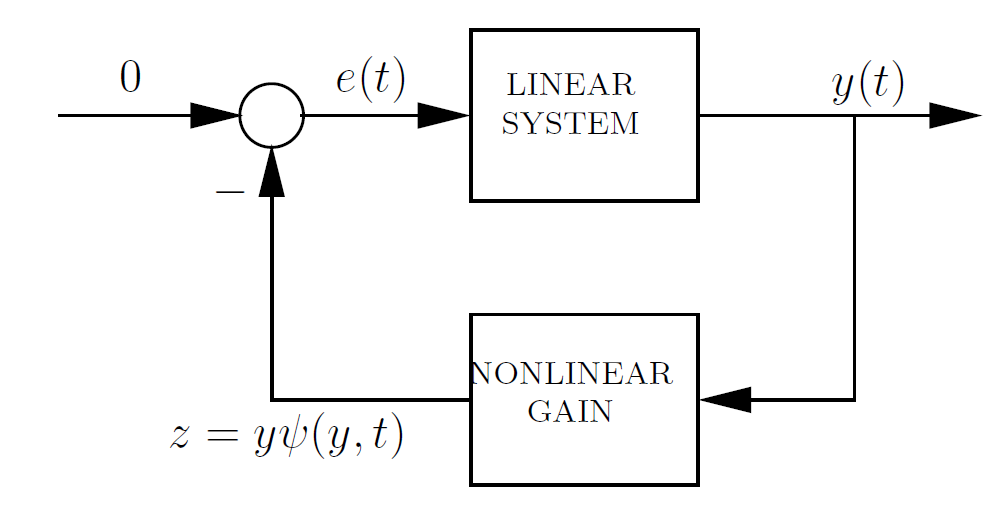
\includegraphics[width=6cm]{bilder/nonlinear_circle_sys.png}
\end{center}
This is a generalization of the Nyquist stability criterion. 
If the nonlinear term $\psi(y,t)$ in above system satisfies $\alpha \leq \psi(y,t) \leq \beta$,
it is called \emph{sector bounded}.

If the Nyquist curve $G(j\omega)$ doesn't penetrate the disc intersecting $-1/\alpha$ and $-1/\beta$,
and encircles it $N_P$ times, where $N_P$ is the number of unstable poles, then
$G(s)$ is stable.
\end{minipage}
\begin{minipage}{5cm}
    \centering
    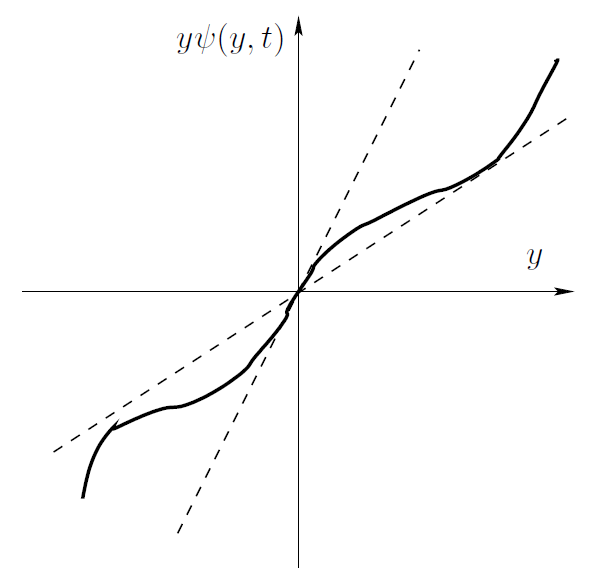
\includegraphics[width=\linewidth]{bilder/nonlinear_sector.png}
\end{minipage}
\begin{minipage}{5cm}
    \centering
    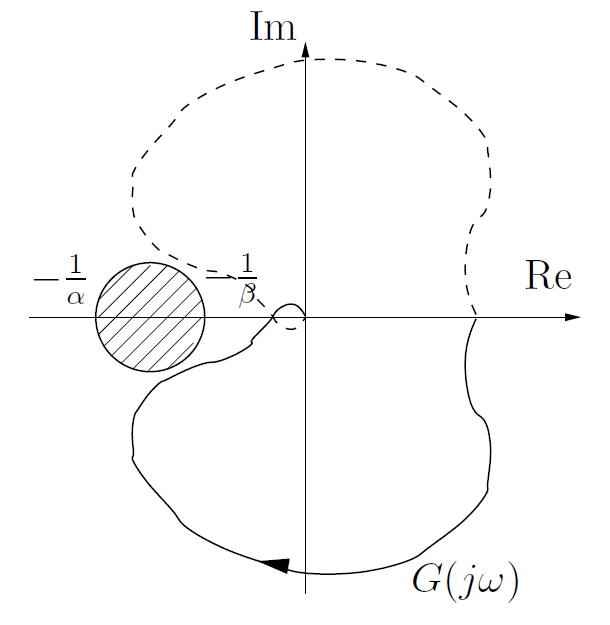
\includegraphics[width=\linewidth]{bilder/nonlinear_circle.png}
\end{minipage}

\subsection{Describing Functions}
\begin{minipage}{10cm}
    The describing method function is a tool to analyze static nonlinearities in a linear control loop.
    If a system reaches a limit cycle, this oscillation leads to a base frequency which can be analyzed.
    It assumes that subharmonic signal parts are small, and thus only looks at the base frequency.
\end{minipage}
\hspace{0.5cm}
\begin{minipage}{8cm}
    \centering
    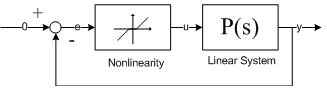
\includegraphics[width=\linewidth]{bilder/nonlinear_system.png}
\end{minipage}

An input signal $e(t) = A \sin(\omega t)$ leads to the output $u_1(t) = C_1 \sin(\omega t + \varphi_1)$.
Similarly to a  transfer function, the \emph{single-input describing function} (SIDF) is
\[
    N(A) = \frac{\tilde{u}_1}{\tilde{e}} = \frac{C_1}{A} e^{j\varphi_1} = \frac{a_1}{A} + j \frac{b_1}{A}
\]
where $a_1$ and $b_1$ are the \emph{Fourier coefficients} of the base frequency $\omega$
and period $T$. They are calculated by
\begin{align*}
    a_1 = \frac{2}{T} \int_0^T u(t) \sin(\omega t) dt &&
    b_1 = \frac{2}{T} \int_0^T u(t) \cos(\omega t) dt &&
\end{align*}
A table of often used describing functions is found in ??
%TODO: add reference to table of describing functions

\begin{minipage}{10cm}
    \paragraph{Loop closure}
    If a limit cycle exists, the loop gain is 1 with a negative feedback. i.e.
    \[
        P(j\omega) N(a) = -1 \qquad \Leftrightarrow \qquad P(j\omega) = -\frac{1}{N(A)}
    \]
    Graphically speaking, if the two curves intersect, a limit cycle condition is met.
    A limit cycle is stable if the plot $-\frac{1}{N(A)}$ intersects $P(j\omega)$ from the right.
    
\end{minipage}
\hspace{0.5cm}
\begin{minipage}{8cm}
    \centering
    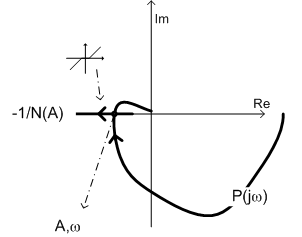
\includegraphics[width=6cm]{bilder/nonlinear_loopclosure.png}
\end{minipage}

%TODO: remove newpage
\newpage
\subsection{Non-Linear Control Methods}

\paragraph{Linearization around an operating point}
Using the Taylor series expansion, a system $\dot{x} = f(x(t),u(t))$ can be rewritten as
\[
    \Delta\dot{x} = A \cdot \Delta x + B \cdot \Delta u
\]
where $A$ and $B$ are the Jacobian matrices
\begin{align*}
    A = \left.\begin{bmatrix}
        \frac{\partial f_1}{\partial x_1} & \frac{\partial f_1}{\partial x_2} & \dots & \frac{\partial f_1}{\partial x_n} \\
        \frac{\partial f_2}{\partial x_1} & \frac{\partial f_2}{\partial x_2} & \dots & \frac{\partial f_2}{\partial x_n} \\
        \vdots & \vdots & \ddots & \vdots \\
        \frac{\partial f_n}{\partial x_1} & \frac{\partial f_n}{\partial x_2} & \dots & \frac{\partial f_n}{\partial x_n} \\
    \end{bmatrix} \right|_{x_0,y_0}
    && \text{and} &&
    B = \left.\begin{bmatrix}
            \frac{\partial f_1}{\partial u_1} & \frac{\partial f_1}{\partial u_2} & \dots & \frac{\partial f_1}{\partial u_n} \\
            \frac{\partial f_2}{\partial u_1} & \frac{\partial f_2}{\partial u_2} & \dots & \frac{\partial f_2}{\partial u_n} \\
            \vdots & \vdots & \ddots & \vdots \\
            \frac{\partial f_n}{\partial u_1} & \frac{\partial f_n}{\partial u_2} & \dots & \frac{\partial f_n}{\partial u_n} \\
        \end{bmatrix} \right|_{x_0,y_0}
\end{align*}
Now all linear techniques can be fully applied, though the operating range is limited.

\paragraph{Compensation of static non-linearities}
Some non-linearities can be compensated by using the inverse function of the non-linearity.
This is often used for actuators and sensors.
Important: the non-linearity must be known and must be invertible.

\begin{center}
    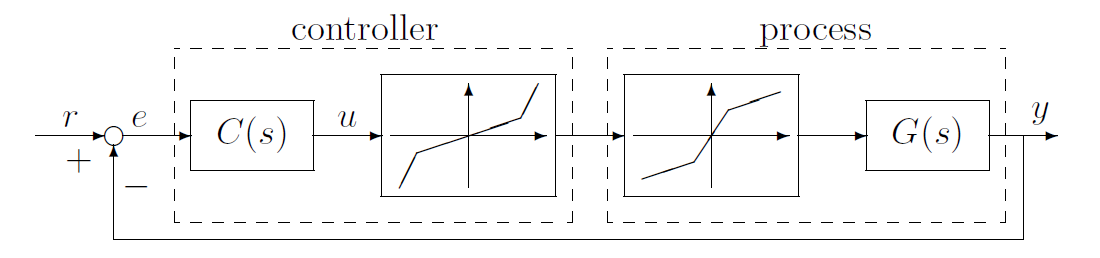
\includegraphics[width=12cm]{bilder/nonlinear_comp.png}
\end{center}

\paragraph{Linearization by local feedback}
If the non-linearity is isolated, it can be controlled by a fast local loop. 
That loop can be treated like a constant gain in a slower outer loop.
For this an additional measurement is needed.
The time scale difference between inner and outer loop must be large enough (5 to 10 times).

\paragraph{Sliding-mode control}
The control is divided into two phases in time: a \emph{reaching phase} where the system
is driven into a \emph{stable} manifold.
In the \emph{sliding phase}, the system slides along the manifold towards the equilibrium.

\paragraph{Relay control}
On-off relais force a system to oscillate in a limit cycle.
The limit cycle can be analyzed using describing functions.

\paragraph{Gain scheduling}
If the process is highly dependent on the operating conditions, these can be measured and
used to parametrize the controller.